% The four internal-propagator types of the in-in (SK) rules: rows are mass types, columns are SK branch combinations.
% The SK branch of a vertex is carried by its fill colour: black = +, white = -, gray = general.
% Full propagators carry the theta pair, cross propagators carry none. The conjugate assignments give
% the same two types.
\documentclass[tikz,border=6pt]{standalone}
\usetikzlibrary{calc,positioning}
\begin{document}
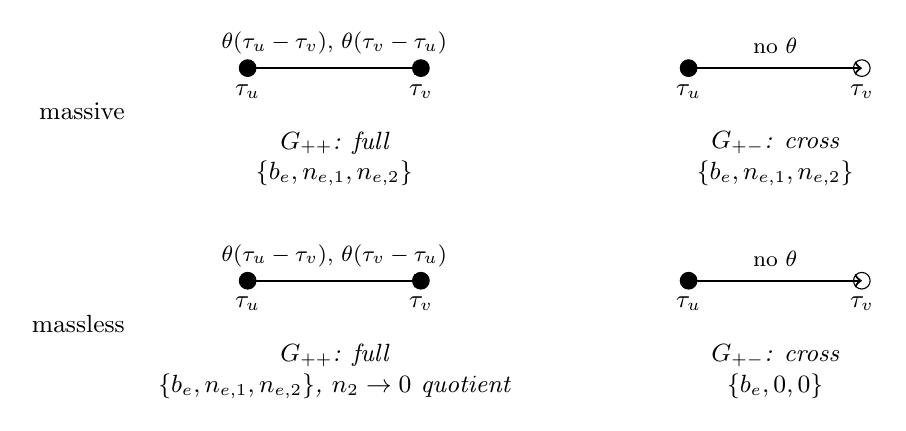
\begin{tikzpicture}[
  every node/.style={inner sep=1.5pt},
  vertexP/.style={circle,fill=black,draw=black,minimum size=6pt,inner sep=0pt},
  vertexM/.style={circle,fill=white,draw=black,minimum size=6pt,inner sep=0pt},
  lab/.style={font=\small},
  plab/.style={font=\small\itshape},
  ttl/.style={font=\small},
]
  % ============ massive / full ============
  \begin{scope}[shift={(0,0)}]
    \node[vertexP] at (0,0) {};
    \node[vertexP] at (2.2,0) {};
    \draw[->,thick] (0,0) -- (2.2,0);
    \node[lab,anchor=north] at (0,-0.15) {$\tau_u$};
    \node[lab,anchor=north] at (2.2,-0.15) {$\tau_v$};
    \node[font=\footnotesize,anchor=south] at (1.1,0.12) {$\theta(\tau_u-\tau_v)$, $\theta(\tau_v-\tau_u)$};
    \node[plab,anchor=north] at (1.1,-0.75) {$G_{++}$: full};
    \node[plab,anchor=north] at (1.1,-1.12) {$\{b_e,n_{e,1},n_{e,2}\}$};
  \end{scope}
  % ============ massive / cross ============
  \begin{scope}[shift={(5.6,0)}]
    \node[vertexP] at (0,0) {};
    \node[vertexM] at (2.2,0) {};
    \draw[->,thick] (0,0) -- (2.2,0);
    \node[lab,anchor=north] at (0,-0.15) {$\tau_u$};
    \node[lab,anchor=north] at (2.2,-0.15) {$\tau_v$};
    \node[font=\footnotesize,anchor=south] at (1.1,0.12) {no $\theta$};
    \node[plab,anchor=north] at (1.1,-0.75) {$G_{+-}$: cross};
    \node[plab,anchor=north] at (1.1,-1.12) {$\{b_e,n_{e,1},n_{e,2}\}$};
  \end{scope}
  % ============ massless / full ============
  \begin{scope}[shift={(0,-2.7)}]
    \node[vertexP] at (0,0) {};
    \node[vertexP] at (2.2,0) {};
    \draw[->,thick] (0,0) -- (2.2,0);
    \node[lab,anchor=north] at (0,-0.15) {$\tau_u$};
    \node[lab,anchor=north] at (2.2,-0.15) {$\tau_v$};
    \node[font=\footnotesize,anchor=south] at (1.1,0.12) {$\theta(\tau_u-\tau_v)$, $\theta(\tau_v-\tau_u)$};
    \node[plab,anchor=north] at (1.1,-0.75) {$G_{++}$: full};
    \node[plab,anchor=north] at (1.1,-1.12) {$\{b_e,n_{e,1},n_{e,2}\}$, $n_2\to0$ quotient};
  \end{scope}
  % ============ massless / cross ============
  \begin{scope}[shift={(5.6,-2.7)}]
    \node[vertexP] at (0,0) {};
    \node[vertexM] at (2.2,0) {};
    \draw[->,thick] (0,0) -- (2.2,0);
    \node[lab,anchor=north] at (0,-0.15) {$\tau_u$};
    \node[lab,anchor=north] at (2.2,-0.15) {$\tau_v$};
    \node[font=\footnotesize,anchor=south] at (1.1,0.12) {no $\theta$};
    \node[plab,anchor=north] at (1.1,-0.75) {$G_{+-}$: cross};
    \node[plab,anchor=north] at (1.1,-1.12) {$\{b_e,0,0\}$};
  \end{scope}
  % row labels
  \node[ttl,anchor=east] at (-1.5,-0.55) {massive};
  \node[ttl,anchor=east] at (-1.5,-3.25) {massless};
\end{tikzpicture}
\end{document}
